\chapter{Memory, caches and the roofline}\label{ch:cache}

Chapters~\ref{ch:gray}--\ref{ch:conv} made the arithmetic cheap. Once arithmetic is cheap, the question becomes: \emph{can the memory system deliver the pixels fast enough?} This chapter is the vocabulary and the measurements for that question.

\section{The memory hierarchy in one picture}

A CPU core cannot compute on data that is far away. Between the core and main memory (DRAM) sit small, fast memories called \textbf{caches}:

\begin{center}
\begin{tabular}{@{}lll@{}}
\toprule
level & typical size (per core / shared) & what it means for us\\
\midrule
registers & 16 vector registers of 32 bytes & the accumulators of the convolution live here\\
L1 data cache & tens of KB per core & a few image rows; latency of a few cycles\\
L2 cache & about 1--2 MB per core on current server CPUs & the $k$ float rows of the convolution ring\\
L3 cache & tens of MB, shared by the cores of a socket & small and medium images\\
main memory & many GB, shared & large images; the bandwidth is the limit\\
\bottomrule
\end{tabular}
\end{center}

The numbers differ per CPU. Never quote them from memory in an interview; print them with \code{lscpu} on the machine you measured on (the Slurm scripts store this in \file{meta.txt}). The sandbox used for the example numbers reports \texttt{L1d 96 KiB (2 instances), L2 4 MiB (2 instances)}, i.e.\ 48 KB and 2 MB per core, and a very large shared L3 that is a property of the virtual machine host. For the cluster partitions the bwHPC wiki lists the CPU types; the cache sizes of those models should be read from \code{lscpu} in your own job output rather than assumed.

Data moves between levels in \textbf{cache lines} of 64 bytes. Reading one byte brings in 64. This is why the library aligns rows to 64 bytes and why the vector loops are written to walk through memory in order: the \emph{hardware prefetcher} recognises a sequential stream and loads the next lines before the program asks for them.

\begin{plain}
\textbf{Library analogy.} The shelf next to your desk (L1) holds a few books. The room's shelves (L2/L3) hold many. The city library (DRAM) holds everything but every trip takes long. Good code reads a book once, uses everything in it, and puts it back. Bad code goes back to the library for every sentence.
\end{plain}

\section{Working sets of the three operations}

The \textbf{working set} is the data that is re-used before it is no longer needed.
\begin{itemize}
\item \textbf{Gray}: nothing is re-used. Each input byte is read once, each output byte written once. The working set is a few lines. It is a pure \emph{streaming} kernel: speed = how fast bytes flow.
\item \textbf{Sobel}: each source row is used by three consecutive output rows. The three rows are read in the same pass; the working set is three rows (a few KB to a few tens of KB, e.g.\ $3\cdot8192$ bytes). It fits in L1/L2 for any realistic width, so every source byte comes from DRAM \emph{once}. Streaming again.
\item \textbf{Convolution}: $k$ float rows of $w+2r$ entries, i.e.\ $4k(w+2r)$ bytes: 148 KB for $w=4096$, $k=9$ (Chapter~\ref{ch:conv}). That is bigger than L1 but fits in L2. The design keeps this ring in cache and streams the image once.
\end{itemize}

\section{Arithmetic intensity and the roofline}

Define the \textbf{arithmetic intensity} $I=\text{operations}/\text{bytes moved}$. A processor has two ceilings:
\[
\text{attainable performance}\;=\;\min\bigl(P_{\text{peak}},\;B\cdot I\bigr),
\]
where $P_{\text{peak}}$ is the peak arithmetic rate and $B$ the memory bandwidth. Plot performance against $I$: a sloped line on the left (memory-bound: more intensity is directly more speed) and a flat roof on the right (compute-bound). This is the \textbf{roofline model}.

\begin{itemize}
\item \textbf{Gray and Sobel} do a handful of integer operations per pixel and move 2--4 bytes per pixel: far left, memory-bound. Once SIMD has removed the instruction overhead, the next ceiling is the memory system.
\item \textbf{Convolution} does $2k^2$ floating-point operations per pixel for the same 2 bytes of traffic: $I=k^2$ operations per byte. Already for $k=3$ it is far to the right of the other two, so it is compute-bound and its limit is the FMA units.
\end{itemize}

\subsection{A measured memory yardstick}

To avoid guessing $B$, the benchmark has an operation \code{copy}: a multi-threaded \code{memcpy} of the same pixel rows into another image. A kernel cannot move bytes faster than a plain copy does, so its \emph{minimum traffic rate} (input bytes read plus output bytes written, counted once) should be compared with the copy's.

\begin{center}
\small
\begin{tabular}{@{}lrrrr@{}}
\toprule
image & threads & copy (GB/s) & gray AVX2 & Sobel AVX2\\
\midrule
2048$^2$ & 1 & 24.6 & 14.5 (59\,\%) & 8.0 (33\,\%) \\
2048$^2$ & 2 & 49.2 & 27.5 (56\,\%) & 15.6 (32\,\%) \\
4096$^2$ & 1 & 25.0 & 14.6 (58\,\%) & 8.4 (34\,\%) \\
4096$^2$ & 2 & 50.4 & 27.7 (55\,\%) & 16.3 (32\,\%)\\
\bottomrule
\end{tabular}
\end{center}


\begin{center}
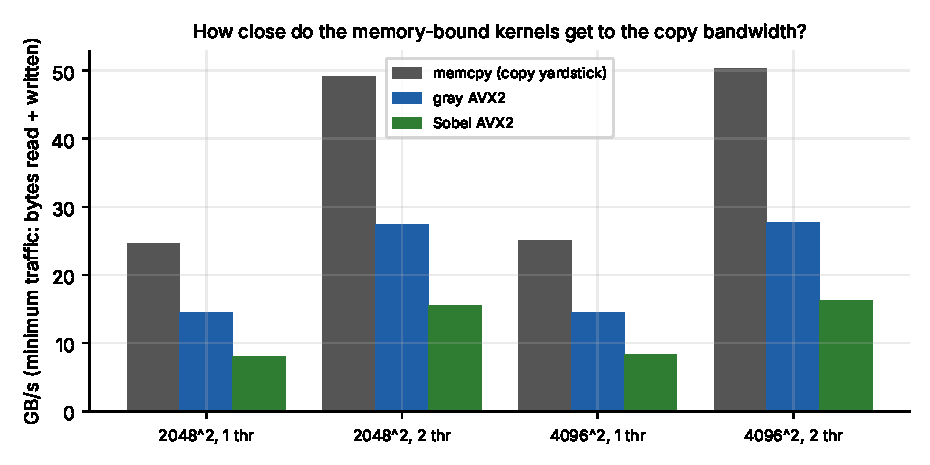
\includegraphics[width=0.85\textwidth]{figures/f_bandwidth.pdf}
\captionof{figure}{Minimum-traffic rate of the AVX2 kernels compared with a plain copy of the same pixels (sandbox VM).}
\end{center}

How to read this honestly:
\begin{itemize}
\item On this machine one thread copies about \copyOneBig\,GB/s from DRAM (images of 2048$^2$ and larger) and two threads about \copyTwoBig\,GB/s, so the sandbox did not saturate its memory with two threads. For small images that fit in cache the copy is faster (\copyOneSmall\,GB/s at 512$^2$), which is the cache hierarchy showing.
\item AVX2 gray reaches about \pctGrayOfCopy\,\% of the copy rate at 4096$^2$, Sobel about \pctSobelOfCopy\,\%. The copy rate counts a read and a write of one byte per pixel; gray reads three bytes per pixel and Sobel reads each pixel through three rows, so neither is expected to reach 100\,\% of that figure with a one-pass design. The conclusion is not ``at the roof'', it is: \emph{within a factor 2--3 of the memory ceiling}, which is where a SIMD kernel that does a little work per byte should be, and far from the instruction-bound regime of the scalar code.
\item This is a measurement on a VM. The same experiment on the cluster (E5 in the scripts) gives \emph{your} yardstick; a different number there is expected and fine.
\end{itemize}

\subsection{Compute side: how close is convolution to the FMA roof?}

The theoretical peak of one core with two 256-bit FMA units is $2\ \text{FMA}\times8\ \text{lanes}\times2\ \text{flop}=32$ flop/cycle. At the nominal 2.1\,GHz of the sandbox CPU that is \nominalPeakGf\,GFLOP/s, and the AVX2 convolution reaches up to \gfAvxMax\,GFLOP/s, about \fracOfNominalPeak\,\% of that figure. Two caveats keep this honest: (1) the clock under load may differ from the nominal value (turbo, or a lower AVX frequency), so the percentage is a rough indicator, not a precise efficiency; (2) the count $2k^2$ flop per pixel counts every tap as one multiply and one add, whether or not the zero weights could be skipped. What the number shows qualitatively: the kernel is limited by the FMA units, not by loads or by the memory system, which is exactly what the design of Chapter~\ref{ch:conv} aims for. Whether the cluster CPUs (Ice Lake, Zen 4) show the same fraction is a measurement for you to make; do not assume it.

\section{Image size and the cache}

\begin{center}
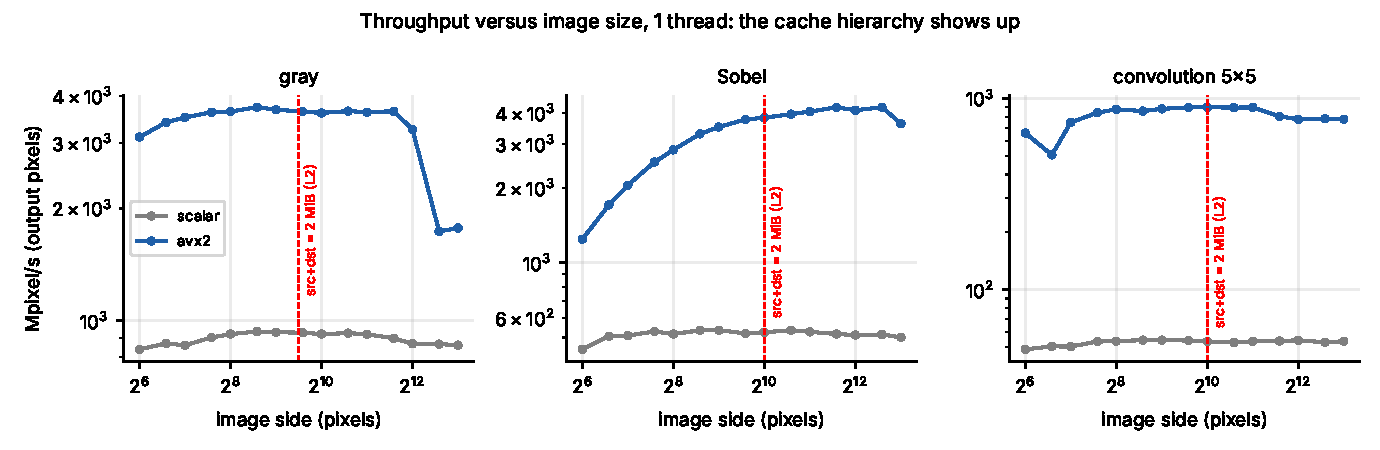
\includegraphics[width=\textwidth]{figures/f_sizes.pdf}
\captionof{figure}{Throughput of scalar and AVX2 versus image side (1 thread). The dashed red line marks the size at which source plus destination together (2 bytes per pixel, 4 for gray) equal 2 MiB, the per-core L2 of this VM.}
\end{center}

Observations in the sandbox data, with the explanation they support:
\begin{itemize}
\item \textbf{Scalar} throughput is flat: it is limited by instructions, and the memory system is never the bottleneck, so image size does not matter.
\item \textbf{AVX2 gray} falls from about \mpixGrayAvxSmall\,Mpix/s at 512$^2$ to about \mpixGrayAvxHuge\,Mpix/s at 8192$^2$ once the data come from DRAM: the SIMD kernel is fast enough to feel the memory.
\item \textbf{AVX2 Sobel} is much less sensitive (\mpixSobelAvxSmall to \mpixSobelAvxHuge\,Mpix/s): it does more arithmetic per byte, so it stays closer to compute-bound.
\item \textbf{Very small images} (below about 100 pixels per side) lose speed to fixed per-call costs: the vector loop only starts after the first pixel and ends before the last, so a larger share of pixels takes the scalar border path.
\end{itemize}

\section{Does the row stride matter?}

Chapter~\ref{ch:images} explained why the library avoids strides that are an exact multiple of 4096 bytes: addresses 4096 bytes apart map to the same cache set, so $k$ rows that are read together can evict each other (\emph{cache associativity conflict} and, on some CPUs, \emph{4K aliasing} between loads and stores). Sobel reads three rows and writes one at the same column offset: that is the pattern that would suffer.

The experiment compares the same operation with stride $=$ width (tight) and stride $=$ width $+64$. Strides of 4096 and 8192 bytes (widths 4096 and 8192) are exact page multiples; widths 1024 and 2048 are powers of two but not page multiples and serve as controls. The last six rows use a 4096-pixel-wide, 512-row image with large kernels.

\begin{center}
\small
\begin{tabular}{@{}llrrr@{}}
\toprule
width & case & stride = width (ms) & stride $+64$ (ms) & power-of-two slower by\\
\midrule
1024 & sobel scalar & 2.17 & 2.08 & +4.6\,\% \\
1024 & sobel avx2 & 0.28 & 0.28 & +0.1\,\% \\
1024 & conv avx2 k=9 & 3.30 & 3.28 & +0.6\,\% \\
2048 & sobel scalar & 8.60 & 8.99 & -4.3\,\% \\
2048 & sobel avx2 & 1.07 & 1.20 & -11.0\,\% \\
2048 & conv avx2 k=9 & 14.05 & 13.99 & +0.4\,\% \\
4096 & sobel scalar & 38.18 & 32.82 & +16.3\,\% \\
4096 & sobel avx2 & 4.40 & 3.99 & +10.4\,\% \\
4096 & conv avx2 k=9 & 56.25 & 55.43 & +1.5\,\% \\
8192 & sobel scalar & 137.21 & 130.16 & +5.4\,\% \\
8192 & sobel avx2 & 18.54 & 18.42 & +0.7\,\% \\
8192 & conv avx2 k=9 & 222.52 & 222.11 & +0.2\,\% \\
4096$\times$512 & conv scalar k=15 & 327.47 & 314.82 & +4.0\,\% \\
4096$\times$512 & conv autovec k=15 & 365.18 & 366.21 & -0.3\,\% \\
4096$\times$512 & conv avx2 k=15 & 17.44 & 17.49 & -0.3\,\% \\
4096$\times$512 & conv scalar k=21 & 680.57 & 637.85 & +6.7\,\% \\
4096$\times$512 & conv autovec k=21 & 693.49 & 699.34 & -0.8\,\% \\
4096$\times$512 & conv avx2 k=21 & 33.03 & 32.74 & +0.9\,\%\\
\bottomrule
\end{tabular}
\end{center}

\begin{center}
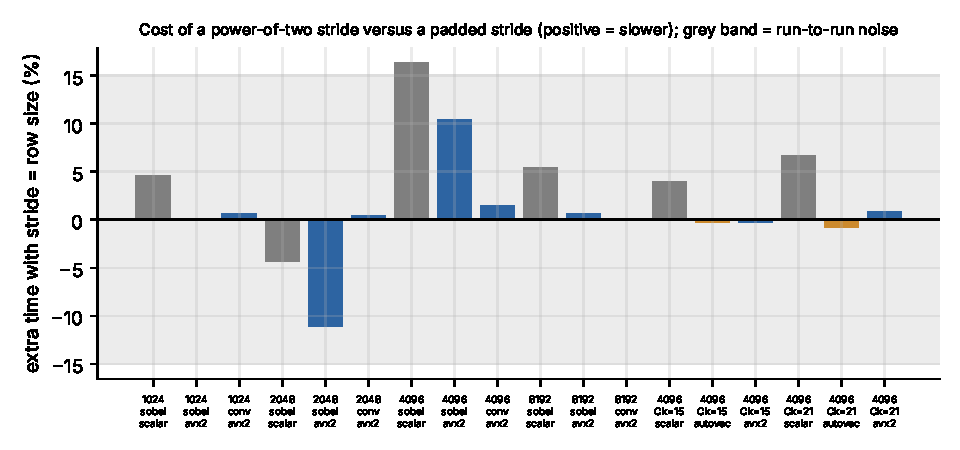
\includegraphics[width=0.95\textwidth]{figures/f_stride.pdf}
\captionof{figure}{Relative cost of the page-multiple stride. Positive values mean the padded stride is faster; the grey band is the run-to-run spread measured in E6 (at least $\pm5\,\%$).}
\end{center}

\begin{warn}[What this experiment does and does not show]
The effect is small and inconsistent: it ranges from about $\strideBestFast\,\%$ to $+\strideWorstSlow\,\%$ (positive: the page-multiple stride is slower), and the run-to-run spread on this VM is of the same order (Chapter~\ref{ch:bench}). The one result in the direction the theory predicts is Sobel at width 4096 (scalar $+16\,\%$, AVX2 $+10\,\%$); but width 8192, which is also a page multiple, shows only $+5\,\%$ and $+0.7\,\%$, width 2048 (not a page multiple) shows the \emph{opposite} sign, and convolution, whose working set is the float ring rather than the image rows, shows no effect beyond $\pm1.5\,\%$ for AVX2. So the honest statement is: \emph{``the padding costs 1.6\,\% memory and removes a failure mode that the theory predicts; on this VM I could not show an effect distinguishable from run-to-run noise.''} Do not claim a measured gain. Repeat E3 on the cluster (the script does), and report what you see, including a null result.
\end{warn}

\section{Other effects the code does not exploit (and you can mention)}

\begin{itemize}
\item \textbf{Tiling / loop blocking over several output rows} would let each loaded source row be used by more than one output row in registers (the convolution here reloads each float row once per output row that uses it: $k$ times). A $2\times$ or $4\times$ row blocking reduces loads; it is the next step toward the FMA roof.
\item \textbf{Non-temporal stores} (\code{\_mm256\_stream\_si256}) skip polluting the cache with output that will not be read again; they help bandwidth-bound writes of large images and hurt small ones.
\item \textbf{NUMA and first touch.} On a two-socket node, memory is attached to a socket. An image allocated and first written by one thread lives near that thread's socket; other sockets read it over a slower link. The scaling script pins threads close together to stay in one place. A full treatment would initialise the image in parallel with the same band layout (``first touch'').
\item \textbf{Huge pages} (2 MB) reduce the number of address translations (TLB misses) for large images.
\end{itemize}

\begin{sound}
``The three kernels sit at very different places on the roofline. Gray and Sobel stream: after vectorization their limit is memory bandwidth, and I measured how close they get with a memcpy of the same pixels. Convolution has $k^2$ operations per byte, so it is bound by the FMA units; the ring of float rows keeps the re-used data in L2, and I measured it at roughly \fracOfNominalPeak{} percent of the nominal peak of one core on my test machine \emph{[yours: on the cluster core]}.''
\end{sound}
